First of all, let us consider the different types of approaches to security protocol analysis. The two categories of techniques are shown in \cref{fig:symbolic-computational-model} and we will proceed to examine them in this chapter.

\begin{figure}[t]
    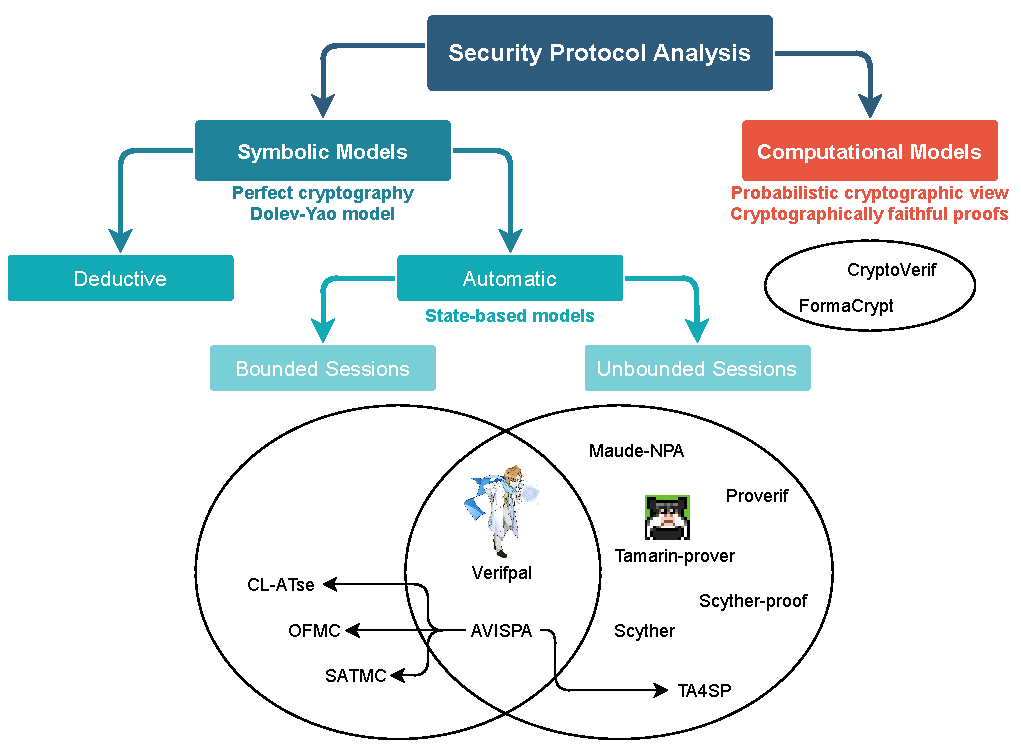
\includegraphics[scale=0.9]{symbolic-computational-model}
    \centering
    \caption{Symbolic and computational models and available tools.}
    \label{fig:symbolic-computational-model}
\end{figure}

In the \textit{symbolic model} (often called Dolev-Yao model) \cite{Dolev-Yao}, the cryptographic primitives are considered as black-box and are represented using function symbols, the messages are terms and the adversary can only use defined primitives. An important aspect to note of this model is that it assumes \textbf{perfect cryptography}. As an example, consider the case in which there are two function symbols (\textbf{enc} and \textbf{dec}, used to encrypt and decrypt), a message \textit{m} and a key \textit{k} and the following equality is defined:

\begin{equation}
\mbox{dec}\left(\mbox{enc}\left(m, k\right), k\right) = m
\end{equation}

Following from the equation $-$ and considering the perfect cryptography assumption $-$ it is possible to decrypt $\mbox{enc}\left(m, k\right)$ if and only if \textit{k} is known \cite{SymbolicComputationalBlanchet}.

In the \textit{computational model} the messages are bitstrings, the cryptographic primitives are functions from bitstrings to bitstrings, the attacker is modeled as a probabilistic Turing machine.
A security property in this model is considered to hold when the probability that it does \textit{not} hold is negligible. For instance, the previously discussed shared-key encryption can be modeled using the same equation. However, the security of encryption is expressed by stating that the attacker has an insignificant probability of breaking the primitive (e.g. decrypting the message without having the key). Security proofs using this model are usually stronger, but this comes to the cost of long, difficult, tedious, highly error-prone proofs (as stated by INRIA researchers \cite{ComputationalAnalysisCryptoSystemsINRIA}). Finally, as pointed to by Blanchet \cite{SymbolicComputationalBlanchet}, the computational model is indeed just a \textit{model} and ignores many aspects of reality and potential attacks, e.g. faulty attacks like the one affecting processors computing RSA signatures \cite{RSAFaultAttack}. 

Of all the tools in \cref{fig:symbolic-computational-model}, we are going to discuss about two automatic tools that employ a symbolic model: \href{https://prosecco.gforge.inria.fr/personal/bblanche/proverif/}{Proverif} and \href{https://tamarin-prover.github.io/}{Tamarin-prover}. We will also refer to Tamarin-prover as Tamarin for brevity. 

We choose to focus on the tools that exploit the symbolic model as it makes it possible to automate proofs. Notice that termination is still not always guaranteed\footnote{It actually depends on the tool. Both Proverif and Tamarin may not terminate. Assuming termination, Proverif proofs may end with an inconclusive result, while Tamarin will always give a proof. Other tools, like Scyther \cite{Scyther}, always terminate by limiting the growth of some parameters. More details about this problem will be discussed in \cref{sec:difficulties-analysis-symbolic}.}. From now on we will always refer to the symbolic model implicitly.

\section{Difficulties in the security protocol analysis in the symbolic model}
\label{sec:difficulties-analysis-symbolic}
Two main problems affect most automatic tools for security protocol analysis: \textbf{infinite state space} and \textbf{undecidability}.

At a high level, to verify a protocol in the symbolic model, one computes the set of terms that the adversary knows. If a certain term does not belong to this set, then the term is considered secret \cite{SymbolicVerificationBlanchet}. The difficulty is that the set of terms is infinite. Specifically, we have to deal with three sources of infinity when analyzing a protocol:
\begin{description}
    \item[\textbf{Messages}] - the adversary can produce messages of any arbitrary size;
    \item[\textbf{Sessions}] - as many attacks are possible only when multiple sessions are executed in parallel, symbolic models often use an unbounded number of sessions;
    \item[\textbf{Nonces}] - if we have an unbounded number of session, then we also must have an unbounded number of nonces to use in those sessions.
\end{description}

There have been various way of tackling this problem:
\begin{itemize}
    \item{It is possible to decide to bound every source of infinity. In this case, the state space is finite. This method was used, for example, by Lowe \cite{LoweNeedhamSchroederPK} and SATMC \cite{SATMC};}

    \item{We can bound the number of executions of the protocol. This still leads to an infinite state space, but \cite{SymbolicModelNPCompleteInsecurity} have shown that insecurity is NP-complete;}
    
    \item{If we do not force any bound, the problem becomes undecidable \cite{SymbolicModelUndecidability1} \cite{SymbolicModelUndecidability2}. As pointed out by \cite{SymbolicVerificationBlanchet}, no automatic tool that always terminates and solves the problem can exist. In general, it is not possible to determine if a certain proof will, eventually, end. \Cref{fig:undecidability} shows the boundary of decidability. As evidenced by the diagram, the problem is decidable if and only if we bound at least two sources of infinity out of three.

    Of course, there are several approaches to confront this problem:

    \begin{itemize}
        \item{Rely on help from the user. This is the approach chosen by Tamarin \cite{TamarinFoundations}, which allows for semi-automatic proofs. In Tamarin, possible messages are ranked by the system, but the user can choose which to solve first;}
        \item{Another possibility is to have tools that may return an inconclusive result $-$ yet are supposed to work correctly in most cases. This is the approach of Proverif \cite{SymbolicVerificationBlanchet};}
        \item{The last approach is to allow non-termination.}
    \end{itemize}
    }
\end{itemize}


\begin{figure}[t]
    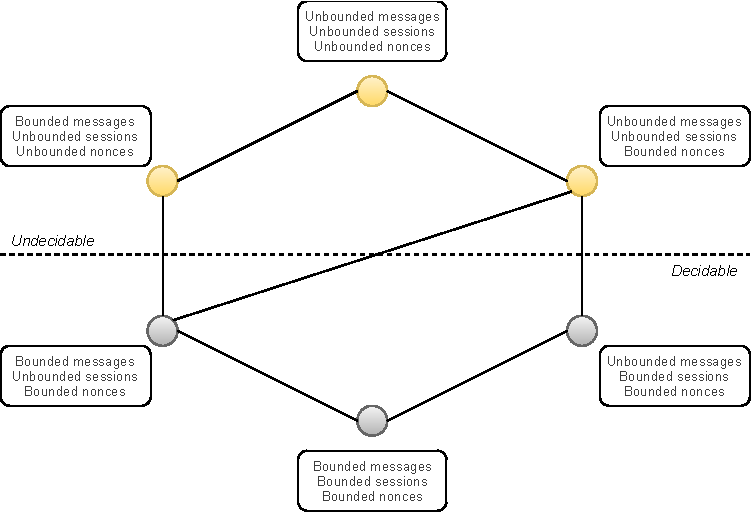
\includegraphics{undecidability}
    \centering
    \caption{Decidability of termination.\\Inspired by a representation from Nicola Vitacolonna.}
    \label{fig:undecidability}
\end{figure}